% !TEX encoding = UTF-8 Unicode
\documentclass[a4paper]{article}

\usepackage{color}
\usepackage{url}
\usepackage[utf8]{inputenc}
\usepackage{graphicx}

\usepackage[english,serbian]{babel}
\usepackage[unicode]{hyperref}
\hypersetup{colorlinks,citecolor=green,filecolor=green,linkcolor=blue,urlcolor=blue}

\usepackage{listings}
\newtheorem{primer}{Primer}[section]

\definecolor{mygreen}{rgb}{0,0.6,0}
\definecolor{mygray}{rgb}{0.5,0.5,0.5}
\definecolor{mymauve}{rgb}{0.58,0,0.82}

\lstset{ 
  backgroundcolor=\color{white},  
  basicstyle=\footnotesize,        
  breakatwhitespace=false,         
  breaklines=true,                 
  captionpos=b,                    
  commentstyle=\color{mygreen},    
  firstnumber=0,                
  frame=single,	                   
  keepspaces=true,                 
  keywordstyle=\color{blue},       
  language=Ruby,                 
  numbers=left,                    
  numbersep=5pt,                   
  numberstyle=\tiny\color{mygray}, 
  rulecolor=\color{black},         
  showspaces=false,                
  showstringspaces=false,          
  showtabs=false,                  
  stepnumber=2,                    
  stringstyle=\color{mymauve},     
  tabsize=2,	                   
  title=\lstname                   
}

\begin{document}

\title{Ruby - dragi kamen, španska serija\\ ili programski jezik?\\ \small{Seminarski rad u okviru kursa\\Metodologija stručnog i naučnog rada\\ Matematički fakultet}}

\author{Vladana Đorđević, Aleksandra Jovičić, Jovana Nikolić, Tijana Tošev\\ vladana1711@gmail.com, jovicicaleksandra96ajs@gmail.com,\\ jovananiki7@gmail.com, tijana.tosev@gmail.com}

%\date{9.~april 2015.}

\maketitle

\abstract{
Šta je to Ruby? Da li je to dragi kamen, telenovela ili programski jezik? Ruby se odnosi na sve tri stvari i, iako su i ostale dve teme bile veoma privlačne, mi smo se odlučili da se u ovom radu fokusiramo samo na programski jezik. Programski jezik  Ruby je objektno-orijentisani skript jezik, ima prirodnu sintaksu, dinamički je i interpretiran. Idejno je nastao 1993. godine, a svetsku slavu stekao je 2006. godine pojavljivanjem razvojnog okruženja Ruby on Rails koje se koristi za razvoj veb aplikacija. U mnoštvu različitih programskih jezika šta je to što Ruby izdvaja od ostalih i zašto treba posvetiti pažnju učenju istog? Ruby odlikuje lakoća učenja, jednostavna sintaksa koja se u velikoj meri poklapa sa sintaksom prirodnog jezika, ali to ne umanjuje njegovu moć. Naprotiv, Ruby je pogodan za primenu u različitim domenima, a to nam upravo govori velika popularnost ovog jezika. Naš cilj je da Vas upoznamo sa njim, prikažemo njegove mogućnosti i da Vas zainteresujemo da ga naučite.}

\addtocontents{toc}{\setcounter{tocdepth}{1}}
\tableofcontents

\newpage
\section{Uvod}
Ovaj rad je namenjen onima koji se tek upoznaju sa Ruby-jem, pa se u skladu sa tim ovde nalaze neke osnove koje su od značaja početnicima. Predstavićemo Vam nastanak i razvoj jezika, namenu, osnovne osobine i specifičnosti kao i razvojna okruženja u kojima se on koristi, uputstva za instalaciju i primere kodova. Moto Ruby zajednice je da članovi budu ljubazni, ugledajući se na tvorca jezika koji je upravo poznat po velikoj ljubaznosti. Stoga, pri učenju jezika možete da računate na pomoć Ruby programera. Naš cilj je da Vam na zanimljiv i pristupačan način približimo ovaj jezik i pomognemo na putu da ga kvalitetno i lako naučite.

%U mnoštvu različitih programskih jezika šta je to što Ruby izdvaja od ostalih i zašto treba posvetiti pažnju učenju istog? Zanimljivo je da je učenje Ruby-ja lako, kako iskusnim programerima, tako i početnicima, jer iako ima korene u mnogim poznatim jezicima, njegova sintaksa je prirodna i u velikoj meri se poklapa sa jezikom koji ljudi koriste. Moto Ruby zajednice je da članovi budu ljubazni, ugledajući se na tvorca jezika koji je upravo poznat po velikoj ljubaznosti. Stoga, pri učenju jezika možete da računate na pomoć Ruby programera. Ovim radom ćemo Vam predstaviti nastanak i razvoj jezika, namenu, osnovne osobine i specifičnosti kao i razvojna okruženja u kojima se on koristi, uputstva za instalaciju i primere kodova. Cilj nam je da Vam prikažemo mogućnosti koje Ruby pruža i da Vas zainteresujemo da ga naučite. 

\section{Istorijski razvoj, uticaj i namena}
%\addtocontents{toc}{\setcounter{tocdepth}{2}}
Ideju za stvaranje Ruby-ja kao novog objektno-orijentisanog (OO) skript jezika, Yukihiro “Matz” Matsumoto, njegov tvorac i softverski inženjer iz Japana, dobio je 23. februara 1993. godine u razgovoru sa kolegom. Pre stvaranja Ruby-ja bio je upoznat sa mnogo drugih programskih jezika, ali njima nije bio zadovoljan. Smatrao je da su bili ružniji, teži, kompleksniji ili jednostavniji nego što je očekivao, pa je želeo je da napravi novi OO skript jezik koji je prirodan, a ujedno i moćan. Matz je želeo da jeziku da ime po dragom kamenu, pod uticajem imena jezika Perl, stoga mu je dao ime Ruby (rubin) jer je to dragi kamen koji odgovara mesecu rođenja jednog njegovog kolege \cite{rubyTalk}\cite{rubyProgLang}.

\subsection{Nastanak i istorijski razvoj}
 
Tokom razvoja Ruby-ja Matz se fokusirao da programiranje učini bržim i lakšim, stoga je sve karakteristike jezika dizajnirao da rade onako kako programeri to očekuju. Upravo to je ono što Ruby čini elegantnim, lakim za korišćenje i zadovoljstvom za programiranje.

Ruby je postao veoma popularan u Japanu 1990-ih godina, međutim, svetsko priznanje dobio je tek 2006. godine pojavljivanjem, danas veoma popularnog, okruženja Ruby on Rails. U decembru 1995. godine objavljen je Ruby 0.95, a u decembru 1996. Ruby 1.0. Svaka verzija se objavljuje na katolički Božić. Najnovija verzija, Ruby 2.6, izbačena je na katolički Božić 2018. godine, dok se verzija 3.0 očekuje 2020. godine \cite{rubyTalk}\cite{rubyProgLang}.

\subsection{Mesto u razvojnom stablu i uticaji drugih programskih jezika}

Kao dugogodišnji ljubitelj OO programiranja, Matz je tražio jezik koji će zadovoljiti njegove kriterijume. Bio je upoznat sa jezicima Perl 4 i Python, ali mu se nisu svideli. Python nije smatrao pravim OO jezikom, jer su OO karakteristike delovale kao dodatak jeziku. Tražio je OO skript jezik, jer mu je izgledao obećavajuće, ali ga nije našao, stoga je odlučio da ga sam napravi. Spojio je delove svojih omiljenih jezika – Perl, Smalltalk, Eiffel, Ada, Lisp i Python. Položaj jezika u današnjem vremenu i njegovu ravnopravnost sa nekim od poznatih programskih jezika možemo videti iz tabele \ref{tab:tabela1} \cite{rubyProgLang}.

\begin{table}[h!]
\begin{center}
\caption{GitHub statistike i godine nastanka programskih jezika}\vspace*{15pt}
\begin{tabular}{|p{1cm}|p{2cm}|p{4cm}|p{2cm}|} \hline
Jezik&Aktivni repozitorijumi&Prosečan broj posmatrača po repozitorijumu& Godina nastanka\\ \hline
C\#&56 062 &4.74&2000.\\ \hline
C++&86 505 &5.77&1983.\\ \hline
Ruby&132 848 &5.92&1995.\\ \hline
Python&164.852 &5.72&1991.\\ \hline
Java&222 852 &6.24&1995.\\ \hline
\end{tabular}
\label{tab:tabela1}
\end{center}
\end{table}
Kao osnovu za Ruby, Matz je koristio programski jezik Lisp. Karakteristike koje su mu se svidele iz drugih jezika je dodavao. OO paradigma je inspirisana jezicima Smalltalk i Perl. Sintaksa je inspirisana Perl-om, a semantika Smalltalk-om, dok je fleksibilnost uzeta iz Python-a. Na slici \ref{fig:sajt2} prikazan je položaj Ruby-ja u razvojnom stablu \cite{rubyTalk}\cite{ruby-doc}.

\begin{figure}[ht!]
\begin{center}
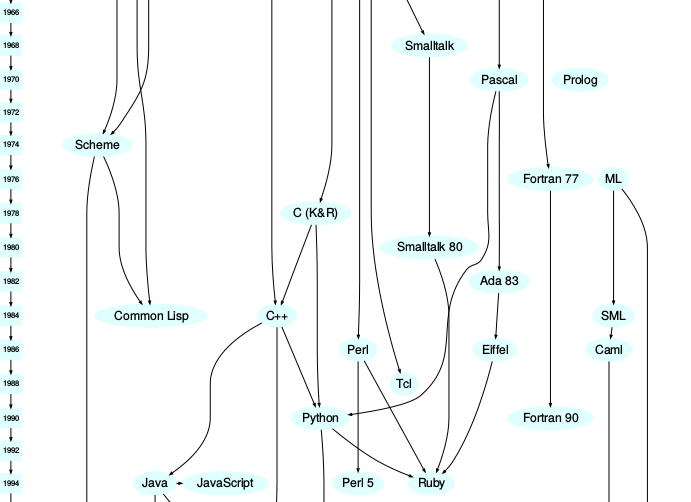
\includegraphics[height=7cm, width=10cm]{SkracenoStablo.png}
\end{center}
\caption{Razvojno stablo}
\label{fig:sajt2}
\end{figure}

\subsection{Namena, svrha i mogućnosti}
Ruby spada u skript jezike i u većini slučajeva se koristi za uopštenu namenu. Važno je napomenuti da je Ruby potpuno besplatan, kao i da ga možemo preuzeti, modifikovati i distribuirati.

Možemo ga koristiti za pisanje veb aplikacija i veb servera, za rad sa bazama podataka, automatizaciju poslova, kreiranje mobilnih/desktop aplikacija i parsiranje. Neki programeri ga koriste i za pisanje programa iz oblasti veštačke inteligencije i mašinskog učenja. Takođe, postoji biblioteka BioRuby koja se koristi u oblasti biologije i medicine.

Poznati projekti koji su implementirani u Ruby-ju su:
\begin{itemize}
	\item \href{https://www.discourse.org/}{Dicourse} - open source platforma za komunikaciju
	\item \href{https://rubyonrails.org/}{Ruby on Rails} - razvojno okruženje za veb
	\item \href{https://www.github.com/}{GitHub} - servis za kontrolu verzije
	\item \href{https://www.airbnb.com/}{Airbnb} - popularna rental-platforma
	\item \href{https://www.hulu.com/tv}{Hulu} - emitovanje televizijskih serija
	\item \href{http://sinatrarb.com/}{Sinatra} - oblasno-specifičan jezik za pisanje veb aplikacija
\end{itemize}


U 2002. godini kada se pojavio Ruby je zauzimao 39. poziciju na TIOBE listi indeksa programskih jezika. Ovaj indeks se računa na osnovu broja pretraga u pretraživačima. Popularnost jezika se menjala kroz godine što možemo zaključiti sa slike \ref{fig:sajt3}, a trenutno se nalazi na 15. poziciji na TIOBE listi.

\begin{figure}[ht!]
\begin{center}
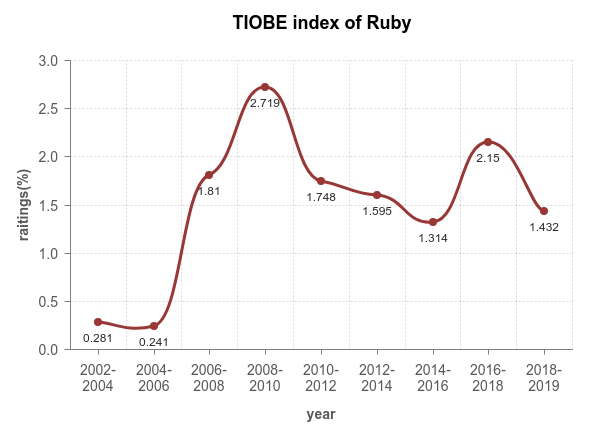
\includegraphics[ height=6cm, width=9cm]{TiobeIndexOfRuby.png}
\end{center}
\caption{TIOBE indeks za Ruby od 2002. godine do danas}
\label{fig:sajt3}
\end{figure}


\section{Osnovne osobine i koncepti}
%\addtocontents{toc}{\setcounter{tocdepth}{1}}
U ovom poglavlju upoznaćemo se sa osnovama jezika, a to počinjemo primerom \ref{matf1}.
\begin{lstlisting}[language=Ruby,caption={Primer ispisa}, frame=single, label=matf1]
	def hello
		# puts naredba moze sadrzati i zagrade
		puts "Hello Matf"
	end
\end{lstlisting}

Ruby poseduje popularne mehanizme poput regularnih izraza, obrade izuzetaka, sakupljače otpadaka i mogućnost pisanja automatske dokumentacije. U nastavku ćemo ukratko opisati neke od najkorišćenijih koncepata jezika.

\subsection{String}
Već u prvom našem programu imamo primer upotrebe Stringa.  Stringovi su jedan od podrazumevanih tipova većine jezika. Nadovezivanje stringova se može izvršiti pomoću operatora “+” ili “\textless\textless”     koji ne menja postojeći String objekat nego dolazi do kreiranja novog. Ukoliko pokušamo nadovezati stringove pomoću “,” tip koji smo dobili zapravo predstavlja objekat klase Array.

Karakterima u stringu možemo pristupati korišćenjem notacije s[i,j], gde je \emph{s} neki string a \emph{i} i \emph{j} indeksi prvog i poslednjeg karaktera podniske koja će biti izdvojena. Neke od ponuđenih klasičnih metoda su \emph{length}(vraća dužinu stringa), \emph{reverse}(obrće redosled čarova u stringu), \emph{swapcase}(menja mala slova u velika i obrnuto), \emph{insert(position, string)} (dodaje nisku na zadatu poziciju u stringu).

\subsection{Array}
Niz je sekvencijalna kolekcija stavki u kojima se svaka stavka može indeksirati. U Ruby-ju jedan niz može da sadrži stavke mešovitih tipova podataka, kao što su stringovi, celi brojevi pa čak i pozivi metoda koje vraćaju neku vrednost. Indeksiranje kreće od nule. Postoji i mogućnost kreiranja matrica kao niza nizova. Moguće je duboko kopiranje gde se promenom jednog niza menja i drugi, novonastali, i plitko gde menjanje jednog ne utiče na drugi niz \cite {HandsOn}. Prvo se vrši pomoću operatora dodele, a drugo pomoću metoda \emph{clone}. 

Niz može da sadrži i \emph{nil} objekte ukoliko neki od članova nije inicijalizovan ili je izvan definisanog opsega. Na primer, za niz n=[1,2,3], n[3]  nam daje vrednost \emph{nil} iz klase \emph{nilClass}. Neke metode koje možemo pozivati nad nizovima su \emph{delete(object)}(briše navedeni element niza), \emph{sort}(sortira niz), \emph{clean}(briše sve elemente), \emph{compact}(vraća niz sa uklonjenim \emph{nil} vrednostima).

\subsection{Hash}
Mogućnost da se umesto brojevnih vrednosti niz indeksira vrednostima drugog tipa je u Ruby-ju omogućena uvođenjem klase Hash. Hash je sličan strukturi koja je poznata i kao mapa u nekim drugim jezicima, gde indeks predstvlja ključ, a pridruženi član indeksa vrednost. Ukoliko za isti ključ definišemo različite vrednosti, ključ  će imati vrednost poslednje definisane vrednosti za taj ključ. 

Kopiranje vrednosti je analogno kopiranju kod nizova. Redosled elemenata u hešu varira u skladu sa verzijom Ruby-ja koja se koristi. U Ruby 1.8 heš se obično skladišti u leksičkom redosledu ključeva, a u Ruby 1.9 heš se čuva u redosledu u kojem su definisani članovi \cite{HandsOn}.

\subsection{IO}
Ruby obezbeđuje klase posvećene rukovanju ulaza i izlaza pomoću klase IO. IO klasa omogućava upravljanje ulazno/izlaznim tokovima bajtova, odnosno otvaranje, zatvaranje, čitanje i pisanje. Klasa File je potklasa klase IO koja poseduje mogućnost navođenja opcija za otvaranje fajla poput \emph{r}(čitanje), \emph{w}(pisanje), \emph{a}(pisanje na kraju fajla). Naredna linija koda otvara tok podataka iz zadatog fajla, čita podatke i ispisuje ih.
\begin{lstlisting}[language=Ruby]
	 IO.foreach("testfile.txt") {|line| print( line ) }
\end{lstlisting}\vspace*{-15pt}

Možemo primetiti da Ruby ima mehanizam koji brine o otvaranju i zatvaranju datoteka umesto korisnika. 

\subsection{Kontrola toka programa i funkcije}
Ruby omogućava brojne načine za pisanje petlji. Imajući u vidu da čitalac poznaje namenu i način funkcionisanja istih, u nastavku predstavljamo moguće sintakse. Takođe, podržan je i koncept grananja naredbama if-then-else.

%kod (petlja i if-else)

U Ruby-ju sve metode uvek vraćaju vrednost s tim da korisnik nije dužan da ih upotrebi. Kada nije navedena povratna vrednost, metode vraćaju rezultat poslednjeg izraza. Prvi navedeni kod u primeru \ref{povVred} vraća vrednost 3, dok je u drugom eksplicitno zadata povratna vrednost.

\begin{lstlisting}[language=Ruby, caption={Primer koda}, frame=single, label=povVred]
	def method1 									def method2
		a = 1													a = 1
		b = 2													b = 2
		c = a + b											c = a + b
	end 															return b
																end
\end{lstlisting}

Neke funkcije mogu imati više povratnih vrednosti i tada je povratna vrednost tipa Array. Objekat tipa Hash takođe može biti povratna vrednost. Argumenti funkcije mogu imati svoje podrazumevane vrednosti navođenjem istih na sledeći način:
\begin{lstlisting}[language=Ruby]
	funkcija( a=10, b=20, c=100)
\end{lstlisting}\vspace*{-15pt}
Značajna novina je da neka funkcija može da ima neodređeni broj argumenata što se postiže dodavanjem zvezdice poslednjem argumentu:
\begin{lstlisting}[language=Ruby]
	funkcija( a=10, b=20, c=100, *d)
\end{lstlisting}\vspace*{-15pt}
Pri pozivu funkcije svi argumenti definisani posle osnovno-definisanih argumenata se smeštaju u niz i u ovom slučaju predstavljaju argument d.

\subsection{Podržane paradigme}
Ruby je prvenstveno predstavnik OO paradigme koja je, za razliku od Jave potpuna, što znači da i primitivni tipovi predstavljaju objekat. Takođe, gotovo sve operacije predstavljaju metode klasa. Kao primer navodimo operaciju množenja “*” u izrazu 5*2=10, koja je metoda objekta 5. Integer 2 je parametar metode, a 10 povratna vrednost.

Iako je OO paradigma glavna odlika Ruby-ja, on podržava i pisanje programa u funkcionalnom i imperativnom stilu. Funkcionalna paradigma se odlikuje prvenstveno mogućnošću pisanja lambda izraza. Sintaksa jednog lamda izraza je sledeca:
\begin{lstlisting}[language=Ruby]
	add = lambda { |x,y| x + y }
\end{lstlisting}\vspace*{-15pt}
Dati metod mozemo pozvati sa \emph{add.call(1,2)}.

Referentna transparentnost gde neku funkciju možemo zameniti sa rezultatom i kompozicija funkcija gde se dve ili više funkcija kombinuje u jednu su još neki od funkcionalnih koncepata koji se mogu koristiti.

Ruby obezbeđuje dobar skup funkcija višeg reda, naročito u klasama Array i Hash, kao što su \emph{each}(za svaki), \emph{select}(izabrati), \emph{push}(dodati na kraj), \emph{pop}(skinuti sa početka), \emph{delete\_if}(izbrisati ako), \emph{map}(mapiranje), \emph{reduce}(sažimanje), \emph{merge}(spajanje), \emph{replace}(zamena). Korišćenje ovih metoda može pomoći da veće probleme brzo svedemo na manje, izbegavajući veći broj imperativnih metoda. Dobijamo čistiji i modularniji kod. U nastavku je dat primer koda \ref{imp} koji ispisuje kvadrate članova niza na klasičan imperativni i elegantan funkcionalni način.
\begin{lstlisting}[language=Ruby, caption={Primer koda}, frame=single, label=imp]
	# imperativni nacin
	i = 0
	while i < array.length do 				
		puts array[i]**2	
	# funkcionalni nacin
	array.collect { | element | element ** 2 }	
\end{lstlisting}\vspace*{-15pt}
\section{Specifičnosti programskog jezika}
Ruby je nastao kao kombinacija različitih programskih jezika, stoga mnoge karakteristike i koncepte deli sa njima. Međutim, poseduje i neke osobine karakteristične samo za njega. U nastavku slede neke od tih specifičnosti.


%Ruby poseduje neke osobine koje ga izdvajaju od ostalih programskih jezika. U nastavku pomenućemo neke od njih. 


\subsection{Oznake promenljivih i simboli}
Promenljive se razlikuju po početnom znaku u imenu. Znakom \$ se predstavljaju globalne promenljive, promenljive instance počinju znakom @, dok klasne promenljive počinju @@ \cite{poignant}.
%Globalne promenljive pocinju sa ... promenljive instane sa ..., dok ...
\begin{lstlisting}[language=Ruby]
	# $x, $iterator, $1
\end{lstlisting}\vspace*{-15pt}
Promenljive koje počinju znakom @ su promenljive instance. One se obično koriste za definisanje atributa.
\begin{lstlisting}[language=Ruby]
	# @x, @y, @width, @height
\end{lstlisting}\vspace*{-15pt}
Promenljive koje počinju sa @@ označava da su to klasne promenljive.
\begin{lstlisting}[language=Ruby]
	# @@x, @@z, @@counter
\end{lstlisting}\vspace*{-20pt}

Simboli su promenljive koje počinju sa “:” i zatim sledi njihov naziv. Nemaju vrednosti ili objekte kao što to imaju promenljive. Koriste se kao konzistentna imena u okviru koda. Razlika je u tome što umesto simbola možemo da navedemo stringove u okviru koda i za svaki navedeni string će se kreirati novi objekat koji će se čuvati u memoriji. Ako koristimo simbole biće inicijalizovani samo jednom. Simboli omogućavaju i čistiji kod. Moguće je konvertovati string u simbol pomoću odgovarajućih metoda, i obrnuto \cite{fromNovice}.

Dva stringa imaju istu vrednost, ali će se posmatrati kao dva različita objekta, dok će u slučaju dva različita simbola oni uvek imati različite vrednosti. Poređenje dva stringa je sporije nego kad poredimo dva simbola i zato se simboli generalno koriste kao ključevi heša.

%\subsection{Sve je True}
%Za razliku od Python-a i ostalih jezika, u Ruby-ju je sve True. Na primer prazna lista ili 0 se smatra %da je False u Python-u, dok je to u Ruby-ju drugačije. Sve osim nil i False se smatra da je True.

\subsection{Blokovi, klasa Proc i lambde}
Svaki kod koji je okružen zagradama “\{\}” ili obuhvaćen ključnim rečima \emph{do} i \emph{end} označava blok. Ideja blokova je da grupišu naredbe koje želimo da se kroz program prosleđuju zajedno. Argumenti blokova su skup promenljivih koje koristimo u bloku i navode se na početku.
\begin{lstlisting}[language=Ruby]
	# {|x, y| x + y}
\end{lstlisting}\vspace*{-15pt}

Blokovi su sintaksne strukture u Ruby-ju i ne smatraju se objektima. Ipak, moguće je kreirati objekat koji predstavlja blok. U zavisnosti kako je taj objekat kreiran razlikujemo \emph{procs} i \emph{lambde}. Klasa Proc omogućava da pozovemo metodu nad njenim instancama (\emph{procs}) i da ih dodelimo promenljivama. Takođe, procs mogu biti i povratne vrendosti metoda. Lambde su Proc objekti koji se više ponašaju kao metode, dok se sami Proc objekti više ponašaju kao blokovi. Razlika se ogleda u tome što lambde proveravaju broj argumenata i drugačiji način tretiraju ključnu reč \emph{return} \cite{rubyProgLang}.

\subsection{Moduli i mixins}
Modul predstavlja grupisane metode, konstante i klasne promenljive. Definisani su kao klase, ali je razlika u tome što oni ne mogu da budu instancirani, kao i da ne mogu biti nasleđeni. To znači da ne postoji višestruko nasleđivanje.

Mixins predstavljaju više pomešanih modula (\emph{eng. mixed in}) i način da se prevaziđe nepostojanje višestrukog nasleđivanja. Omogućavaju kontrolisan način dodavanja funkcionalnosti klasama. Moduli ne mogu da imaju instance zato što nisu klase, ali možemo da uključimo module u okviru neke klase. Na taj način svi metodi modula su na raspolaganju kao metodi u datoj klasi. Zapravo, pomešani moduli se ponašaju kao superklase \cite{ruby-doc}.

Primerom \ref{mixins} pokazujemo upotrebu \emph{mixin Comparable} koji može da se koristi za dodavanje operatora poređenja (\textless , \textgreater , \textgreater =, \textless =, ==) i metode \emph{between?(min,max)} nekoj klasi. Kako bi ovo radilo \emph{Comparable} pretpostavlja da klasa koja ga koristi ima definisan operator  “\textless =\textgreater”. Konačno, potrebno je da definišemo jedan metod koji implementira operator “\textless =\textgreater” i uključimo \emph{mixin Comparable} kako bismo dobili dodatnih šest metoda poređenja besplatno.
\begin{lstlisting}[language=Ruby, caption={Primer koda}, frame=single, label=mixins]
	class Primer
		include Comparable
		attr :str
		def <=>(other)
			str.size <=> other.str.size
		end
		def initialize(str)
			@str = str
		end
		def inspect
			@str
		end
	end
	
	s1 = Primer.new("pas")
	s2 = Primer.new("rubin")
	s3 = Primer.new("tacka")
	
	puts s1 < s2 				# => true
	puts s3.between?(s1, s2)	# => true
	
\end{lstlisting}\vspace*{-15pt}

\subsection{Transparentnost i fleksibilnost}
Ukoliko je potrebno odratiti složen posao u što manje linija koda i na jednostavnoji način pogodno je koristiti Ruby. %Mnogi će izabrati Ruby za neke poslove zato što će neki posao koji bi inače zahtevao nekoliko dana biti završen kroz nekoliko sati. 
Jedna od odlika Ruby-ja je njegova transparentnost. Pod tim se podrazumeva da za rešenja naših problema ne moramo imati mnogo dokumentacije kako bismo odradili neke jednostavne stvari. Pomoću ovog programskog jezika možemo da direktno izrazimo ideje i dizajne rešenja problema, i to na elegantan način. Sve ovo znači da ćemo kucati brže, kao i da su naši kodovi čitljiviji i lakše održivi. U primeru koda \ref{httpkod} povezujemo se na HTTP server i dohvatamo telo veb strane kao string objekat koji ispisujemo na standardni izlaz \cite{poignant}.
\begin{lstlisting}[language=Ruby, caption = "Primer koda", label=httpkod]
	require 'net/http'
	Net::HTTP.start ('www.ruby-lang.org',80) do  |http|
		print (http.get('/en/about/license.txt').body)
	end
\end{lstlisting}\vspace*{-15pt}


\section{Razvojna okruženja}
Ruby ima mnoštvo razvojnih okruženja, posebno u domenu razvoja veb aplikacija. Najpoznatija okruženja za razvoj veb aplikacija su svakako Ruby on Rails, koji je najpopularniji u ovom domenu, zatim Sinatra, Padrino, Hanami (ex. Lotus), NYNY, Cuba, Crepe, Grape, Nancy, Hobbit, Scorched, Rack.Bez obzira na veliki broj okruženja, odlučili smo da posebnu pažnju posvetimo Ruby on Rails koji je i dalje najdominantniji među pomenutim.
\subsection{Ruby on Rails}
Ruby on Rails je jedno od najpopularnijih razvojnih okruženja za razvoj veb aplikacija. Zapravo, njegovim pojavljivanje, Ruby je postao svetski poznat jezik. Napravljeno je da učini programiranje veb aplikacija lakšim praveći pretpostavke o tome šta je svakom programeru potrebno da bi počeo. Omogućava da se napiše manje koda, a da se pritom ostvari više nego u mnogim drugim jezicima i okruženjima. Iskusni Rails programeri kažu da čini razvoj veb aplikacija zabavnijim \cite{rubyOnRails}.

Rails pravi pretpostavke o tome da postoji “najbolji” način da se nešto uradi i dizajniran je tako da podstiče programera da koristi taj način, a u nekim slučajevima i da ga obeshrabri da koristi alternativne načine.  Rails ima dva osnovna principa - "Dogovor umesto konfiguracije" (eng. Convention over configuration) i "Ne ponavljaj se" (eng. Don't repeat yourself). To znači da okruženje obezbeđuje šablone i očekuje se da će ih programer koristiti bez izmena, kao i da će otklanjati kod koji se ponavlja. Ovaj pristup razvoju veb aplikacija funkcioniše veoma dobro kod većine ljudi, međutim, potrebno je napraviti kompromis. Da bi se obezbedio sistem koji funkcioniše bez konfiguracija i koda koji se ponavlja, Rails u velikoj meri koristi dinamičke karakteristike Ruby-ja. Klase se konstruišu pri izvršavanju a metode se dinamički generišu. Programeri koji nauče da pravilno koriste ovo okruženje verovatno će otkriti ogroman porast produktivnosti. Međutim, ukoliko su uporni u nameri da donesu stare navike iz drugih jezika u okruženje Rails i pokušavaju da koriste šablone koje su naučili negde drugde, mogu imati lošije iskustvo \cite{rubyOnRails}\cite{specDynTech}.


Mnoge poznate aplikacije napisane u Ruby-ju su napravljene upravo pomoću Ruby on Rails okruženja koje je prvi put objavljeno 25.10.2004. Poslednja verzija 5.2.2.1 objavljena je u martu 2019. godine. Rails je softver otvorenog koda, čijem razvoju je doprinelo više od 4500 ljudi, a preuziman je skoro 166 miliona puta \cite{rubyToolbox}.

\begin{figure}[ht!]
\begin{center}
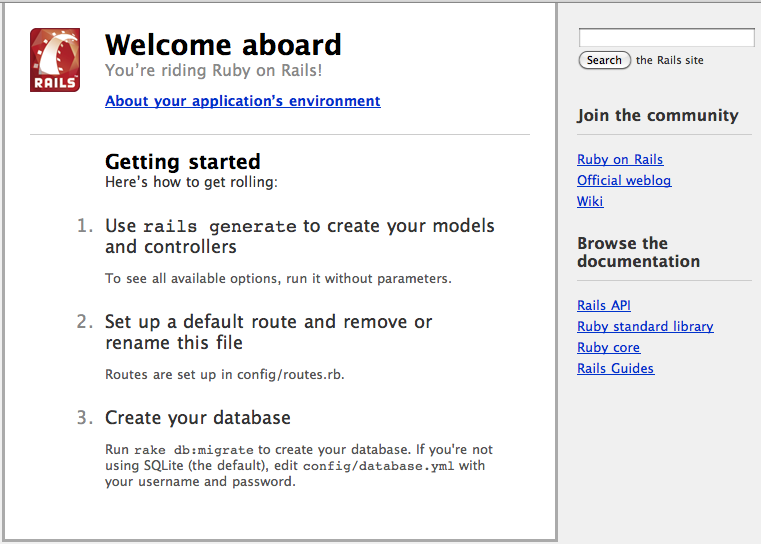
\includegraphics[ height=5cm, width=9cm]{rails_welcome.png}
\end{center}
\caption{Razvojno okruženje - Ruby on Rails}
\label{fig:sajt4}
\end{figure}

\section{Instalacija i uputstvo za pokretanje programa na Linux i Windows operativnim sistemima}
%\addtocontents{toc}{\setcounter{tocdepth}{2}}
Instalacija i izvršavanje standardne implementacije programskog jezika Ruby je podržana na različitim operativnim sistemima. Ne zahteva mnogo napora tako da nije izazov za korisnike i brzo i efikasno se odrađuje.  U narednom delu prikazujemo slučajeve kod operativnih sistema Linux i Windows.

\subsection{Instalacija}
Najjednostavniji način za instalaciju Ruby programskog jezika na Linux operativnom sistemu(distribucija Debian i Ubuntu) je korišćenjem \emph{apt} menadžer paketa.
Prvo, ažuriramo listu dostupnih paketa:
\begin{lstlisting}[language=bash]
  $ sudo apt update
\end{lstlisting}\vspace*{-15pt}
Instaliramo Ruby naredbom:
\begin{lstlisting}[language=bash]
  $ sudo apt install ruby-full
\end{lstlisting}\vspace*{-15pt}
Radi provere da li je instalacija uspela koristimo sledeću naredbu koja nam prikazuje verziju Ruby programskog jezika:

\begin{lstlisting}[language=bash]
  $ ruby --version
\end{lstlisting}\vspace*{-15pt}
Treba da se dobije izlaz nalik ovom:
\begin{lstlisting}[language=bash]
  ruby 2.3.1p112 (2016-04-26) [x86_64-linux-gnu]
\end{lstlisting}\vspace*{-15pt} 

Naredbe za instalaciju razlikuju se na različitim distribucijama Linuxa. U primeru su navedene one koje se odnose na distribuciju Debian i Ubuntu. Za korišćenje Fedora distibucije umesto \emph{apt} možemo koristiti \emph{yum} menadžer paketa.

Program RubyInstaller je jedan od načina instalacije Ruby-ja na Windows operativnim sistemima koji se može naći na adresi \url{http://rubyinstaller.org/downloads/}. Prilikom njegovog pokretanja moramo prihvatiti licencu i izabrati putanju instalacije.Paketi za instalaciju za ostale operativne sisteme se mogu naći na adresi \url{http://www.ruby-lang.org/en/downloads} \cite{rubyLang}.
\subsection{Pokretanje programa}
Kod napisan u Ruby se može pokrenuti na tri različita načina. Prvi je kada kreiramo datoteku sa programskim kodom i pokrenemo je naredbom:
\begin{lstlisting}[language=bash]
  $ ruby primer.rb
\end{lstlisting}\vspace*{-15pt}
Kada nam je potrebno izvršavanje nekoliko linija koda možemo pokrenuti i interaktivnu konzolu Ruby jezika naredbom:
\begin{lstlisting}[language=bash]
  $ irb
\end{lstlisting}\vspace*{-15pt}
Moguće je izvršiti kod koji se piše zajedno sa pozivom interpretera korišćenjem opcije \emph{-e}. Ovde se kod prosleđuje kao argument:
\begin{lstlisting}[language=bash]
  $ ruby -e "puts 'Zdravo!'"
\end{lstlisting}\vspace*{-15pt}

\section{Primer jednostavnog k\^{o}da}
Naredni  primer koda \ref{kod1} prikazuje kako je moguće pristupiti objektu klase String, u našem primeru pod imenom \emph{linija}, preko drugog objekta klase String, u primeru ‘Ruby’. Ukoliko se vrednost ‘Ruby’ poklapa sa nekim delom vrednosti \emph{linija} onda će se vratiti objekat klase String sa vrednošću ‘Ruby’, u suprotnom se vraća \emph{nil}. Takođe, u primeru se vidi da smo ovu mogućnost jezika iskoristili da promenimo vrednost ‘Ruby’ u ‘*Ruby*’.
\begin{lstlisting}[language=Ruby, caption={Prvi primer koda}, frame=single, label=kod1]
linija = "Boja i ukus cokolade Ruby poticu od zrna kakaovca"

# Izlaz "BOJA I UKUS COKOLADE *RUBY* POTICU OD ZRNA KAKAOVCA"
linija['Ruby'] = "*Ruby*"
puts linija.upcase

# pet puta vrsi ispis "Boja i ukus cokolade *Ruby* poticu od zrna kakaovca"
5.times { puts linija }
\end{lstlisting}

Primer koda \ref{kod2} nam pokazuje da Ruby zna šta programer hoće čak i kada izvršava matematičke operacije nad objektom klase Array. Ispisuje elemente koji predstavljaju razliku dva objekta klase Array.
\begin{lstlisting}[language=Ruby, caption={Drugi primer koda}, frame=single, label=kod2]
#Izlaz "Treba nam jos da bi sve bilo posadjeno:
#		kruska
#		sljiva
#		breskva"

sadnice  = %w[ jabuka kruska sljiva tresnja breskva]
zasadjeno = %w[tresnja jabuka]
puts "Trebaju nam jos i naredne sadnice" +
     "da bi sve bilo posadjeno:",
     sadnice - zasadjeno
\end{lstlisting}

\section{Zaključak}
Ruby je osmišljen sa namerom da usreći programera koji ga koristi, ali pored toga pruža ogromne mogućnosti u različitim domenima razvoja softvera i poseduje veliku moć. Stoga, nije iznenađenje što je za veoma kratko vreme postao popularan i cenjen širom sveta. Trenutno je najzastupljeniji u izradi veb aplikacija, zahvaljujući Ruby on Rails okruženju, međutim, mi verujemo da će biti sve više korišćen i u ostalim domenima, zbog svoje pogodnosti za opštu upotrebu. Ideja ovog rada bila je da približi Ruby zainteresovanima, da im predstavi njegove karakteristike, namene, primenu, ne zalazeći previše u detalje, a opet obezbeđujući dovoljno informacija da se Ruby dobro razume. Nadamo se da smo u tome uspeli i da će Ruby zajednica nastaviti da se povećava.


%Osim toga što je namenjen da usreći programera koji ga koristi, takođe je upotrebljiv u različitim oblastima primene i poseduje veliku moć. Zbog toga je za veoma kratko vreme postao veoma popularan i cenjen širom sveta. Ovim radom smo početnicima obezbedili osnovne informacije dovoljne za razumevanje karakteristika i namene Ruby-ja, ne zalazeći u detalje. 

\addcontentsline{toc}{section}{Literatura}
\appendix
\bibliography{literatura} 
\bibliographystyle{unsrt}



\end{document}
